% conclusion
In this thesis, we variationally optimized ground states within manifolds of isometric tensor network states and, oriented towards the tangent space, quasiparticle excitations on top. In the following, we provide a concise summary of the central components: the ansätze, the corresponding optimization algorithms, and the main numerical results for the TFI model. Parts 1) and 2) reproduce well-established methods, while part 3) contains the newly developed bulk-weighted boundary compression and the quasiparticle excitation ansatz for isoPEPS:
\begin{enumerate}
	\item[1)] Uniform matrix product states (uMPS) \\[0.3em]
	The translation invariant state \eqref{eq:umps} on an infinite chain is completely characterized by a single rank-3 tensor. Within the gauge freedom \eqref{eq:umps_gauge}, via iterative positive QR decompositions \eqref{eq:iterative_qr}, we can isolate a normalized center tensor that is surrounded by isometries \eqref{eq:umps_canonical_form}. To optimize for the ground state, the VUMPS algorithm (\ref{item:vumps_1}--\ref{item:vumps_3}) forces the residual of the Schrödinger equation---which is not exactly solvable within the manifold---to be orthogonal to the tangent space. The latter serves as variational space for quasiparticle excitations \eqref{eq:uexcitation_ansatz} against the correlated ground state vacuum. They arise from a superposition of local tensor perturbations, which are gauged \eqref{eq:uexcitation_gauge} such that orthogonality to the ground state \eqref{eq:excitation_gs_overlap} and identity norm matrix \eqref{eq:excitation_overlap} are ensured. Due to translation invariance, we can impose a well-defined momentum that gives direct access to the dispersion relation (figure \ref{fig:uexcitations_dispersion}). In the boundary terms of all effective Hamiltonians, we deal with infinite geometric sums (\ref{eq:Lh}, \ref{eq:mixed_geometric_sum}) of transfer matrices \eqref{eq:transfer_matrix}. To compute them, we make explicit use of the primitivity property \eqref{eq:primitive_transfer_matrix}.
	
	\item[2)] Matrix product states (MPS) \\[0.3em]
	Compared to 1), we restrict the chain to a finite length and make the tensors site-dependent \eqref{eq:mps}. For OBC, the canonical form \eqref{eq:canonical_form_mps} can be reached via two half-sweeps of LQ \eqref{eq:mps_canonical_form_lq} and singular value \eqref{eq:mps_canonical_form_svd} decompositions. The DMRG algorithm (\ref{eq:dmrg}--\ref{eq:dmrg_mps_update}) finds a faithful ground state approximation by solving the effective eigenvalue problem for two tensors at a time, followed by SVD truncation and shift to the next site. Completely analogous to uMPS, but without the explicit plane wave coefficient, the excitation ansatz \eqref{eq:excitation_ansatz} superposes local tensor perturbations and gauges them \eqref{eq:excitation_gauge} so that they are orthogonal to the ground state and pairwise to each other \eqref{eq:emps_orthogonality}. By choosing PBC for the Hamiltonian, momentum can be restored as a good quantum number, either (a) after or (b) together with energy optimization (figure \ref{fig:excitations}). For OBC, the excitations describe standing wave configurations with nodes at the boundaries (figure \ref{fig:excitations_local_energies}). Environments (\ref{eq:L_LB_R_RB}, \ref{eq:local_energies_boundary_tensors}) are contracted by recursively summing up the tensors that (i) newly apply a perturbation to the trivial boundary, and (ii) transfer the boundary of all perturbations that already have been applied.
	 
	\newpage
	\item[3)] Isometric projected entangled pair states (isoPEPS) \\[0.3em]
	On a diagonal square lattice with OBC \eqref{eq:diagonal_square_lattice_2}, we impose the isometric conditions (\ref{eq:AL}--\ref{eq:CD}) on a strict subset \eqref{eq:iso_peps} of 2D tensor network states \eqref{eq:peps}. The orthogonality column can be shifted approximately with the YB move \eqref{eq:YB} and allows to implement a squared variant (\ref{eq:dmrg2_column_update}, \ref{eq:dmrg2_two_site_dmrg}) of the successful 1D DMRG algorithm. The boundaries \eqref{eq:Lh_bMPS} can in general only be contracted approximately. Seeing the two legs that stick out on each site as one "physical" leg of dimension $D_{\text{max}}^2$, this corresponds to a bMPS compression. To be precise, to an additive compression of the two terms (i) $(L_h^{\text{new}} \vert$ that newly applies a column MPO to the identity boundary, and (ii) $(L_h^{\text{transfer}} \vert$ that transfers the boundary of all previously applied column MPOs. The standard procedure is given by a variational sweep \eqref{eq:bc_update_theta2} over a bMPS $( L_h \vert$ with fixed bond dimension $\chi_{\text{max},b}$. In this way, all states in the variational space of dimension $D_{\text{max}}^{2(2L_y-1)}$ are weighted equally, with no regard to the bulk of the isoPEPS. Consequently, the compression fidelity worsens when capturing a smaller fraction of the space, as happens when increasing $D_{\text{max}}$ while scaling $\chi_{\text{max},b} = 6D_{\text{max}}^2$.
For $D_{\text{max}} > 4$, this deterioration becomes evident both in the energy expectation value (figure \ref{fig:bc}) and its minimization with $\text{DMRG}^2$ (figures \ref{fig:dmrg2_3.5_1}--\ref{fig:dmrg2_3.0_2}). These findings motivated us to propose a new \textbf{bulk-weighted boundary compression} (\ref{eq:bulk_weighted_bc}--\ref{eq:bulk_weighted_bc_last_site}). It requires the target bMPS $( L_h \vert$ and the sum to be compressed---namely, $(L_h^{\text{new}} \vert + (L_h^{\text{transfer}} \vert$---to approximately have the same expectation value with the double orthogonality column $\vert C \overline{C} )$ positioned right next to them. Due to the isometric structure of the isoPEPS, the latter contains the entire information about the bulk. With this compression method we reach significantly lower energy errors when computing the expectation value (figure \ref{fig:bc}) or running $\text{DMRG}^2$ (figures \ref{fig:dmrg2_3.5_1}--\ref{fig:dmrg2_3.0_2}). \\
To create \textbf{isoPEPS quasiparticle excitations}, we start from the tangent space of a ground state $\ket{\psi(A_L, C)}$ \eqref{eq:iso_peps_AL_C}. A subtle difference to MPS is given by the fact that the orthogonality column $C$ remains nontrivial when located to the right of all left isometric site tensors. This requires including the derivative with respect to each of its components when forming the tangent space vector \eqref{eq:iso_peps_tangent_vector}. In a fashion analogous to MPS, we parametrize the perturbation tensors \eqref{eq:e_iso_peps_VL_plus} and \eqref{eq:e_iso_peps_VD} such that all desired orthogonality conditions \eqref{eq:e_iso_peps_properties} are satisfied. While for MPS this is exactly covered by the gauge freedom, our isoPEPS parametrization does not span the full tangent space. It projects out more directions than strictly necessary to remove the obvious zero-modes \eqref{eq:e_iso_peps_gauge}, although the closed loops in the isoPEPS bonds may allow additional gauge transformations that are not as straightforward to write down and depend on the specific representation of the reference ground state. In any case, by enforcing the orthogonality relations \eqref{eq:e_iso_peps_properties}, we ensure that the map $X \mapsto \ket{\psi(X; A_L, C)}$ \eqref{eq:e_iso_peps} is injective, making the variational problem well-defined. We solve it (i) via overlap with exact wavefunctions \eqref{eq:_excitation_overlap_wavefunction} or MPS \eqref{eq:_excitation_overlap_mps}, and (ii) by diagonalization of the effective Hamiltonian \eqref{eq:Heff_B}. The resulting states provide good approximations of the low-energy standing wave excitations in the paramagnetic phase of the TFI Hamiltonian (figures \ref{fig:single_particle}--\ref{fig:excitations_effective}). \\[0.5em]
\end{enumerate}


% outlook
\noindent \underline{Reaching higher bond dimensions for excitations} \\[0.5em]
Using our current implementation of the effective Hamiltonian \eqref{eq:Heff_B}, we can optimize the ansatz only up to $D_{\text{max}} = 3$ on the available hardware. Memory and runtime costs could potentially be reduced by improving the boundary compressions \eqref{eq:RB} and \eqref{eq:LBh}. At present, we perform them variationally and treat the different contributions in a unified way, by contracting them into a double-site shape and performing QR decompositions before compressing their sum. For the third term in \eqref{eq:LBh}, for instance, this scales with $\mathcal{O}( D_{\text{max}}^6 \chi_{\text{max}, b}^3 \chi_{\text{max}, c}^3)$ in runtime and with $\mathcal{O}( D_{\text{max}}^4 \chi_{\text{max}, b}^2 \chi_{\text{max}, c}^2)$ in memory per site. A more efficient approach would be to introduce individual environments for each overlap with the bMPS being swept over. \\
In addition to these improvements within the variational compression scheme, it is worthwhile to investigate whether the new bulk-weighted compression, suitably adapted, also brings an advantage for excitations. For boundaries containing a $B$-column in the ket, one could form the expectation value with a single ground state orthogonality column in the bra. \\[1em]

\noindent \underline{Application to conventional MM isoPEPS} \\[0.5em]
Originally, isoPEPS were introduced for the conventional, unrotated square lattice \cite{zaletel2020isometric}:
\begin{equation}
	\ket{\text{isoPEPS}} = \raisebox{-0.5\height}{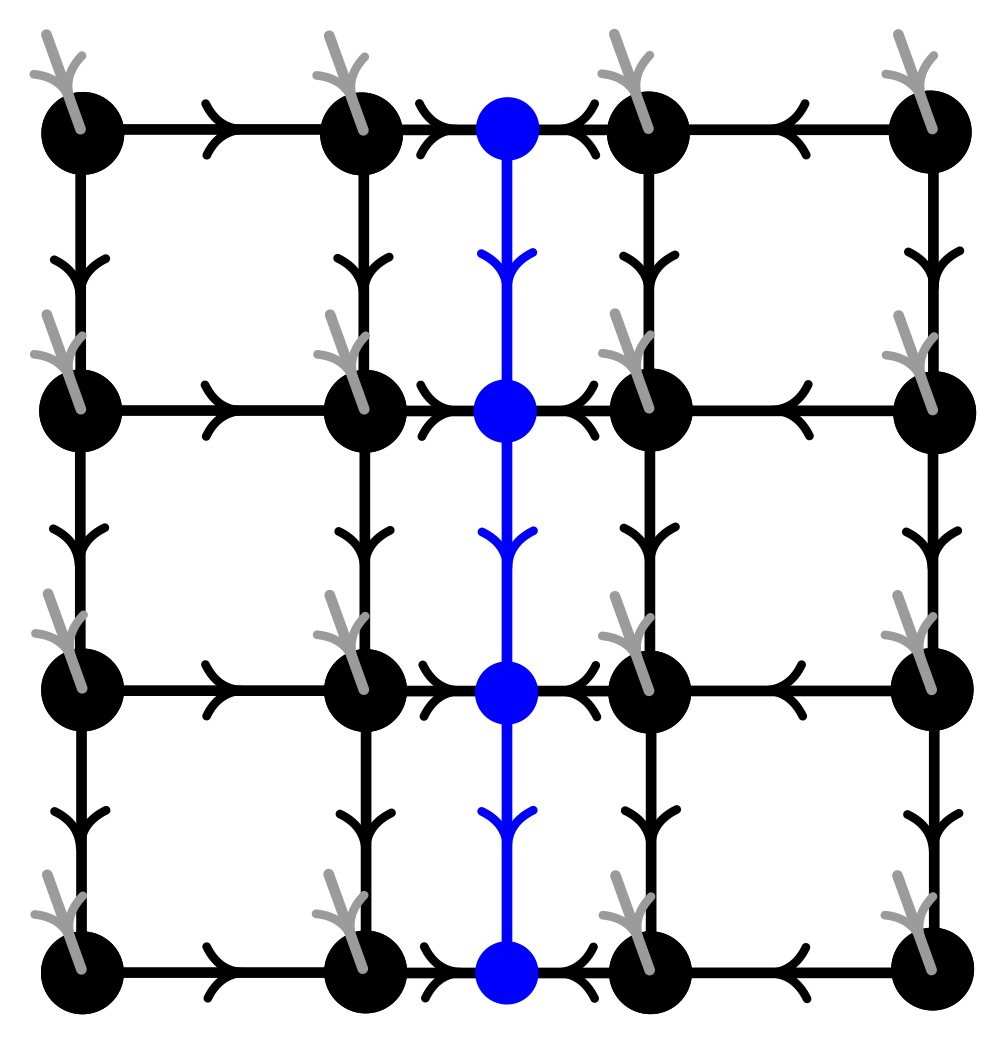
\includegraphics[height=3.5cm]{mm_iso_peps.png}} \:.
\end{equation}
Here, the orthogonality column is shifted with a scheme dubbed the \textit{Moses move} (MM). It merges $C^{[x]}$ with the adjacent isometric column $A_R^{[x+1]}$ into $A_C^{[x+1]}$ and then splits the latter back into two columns $\tilde{A}_L^{[x+1]}$, $\tilde{C}^{[x+1]}$: 
\begin{equation}
	\raisebox{-0.5\height}{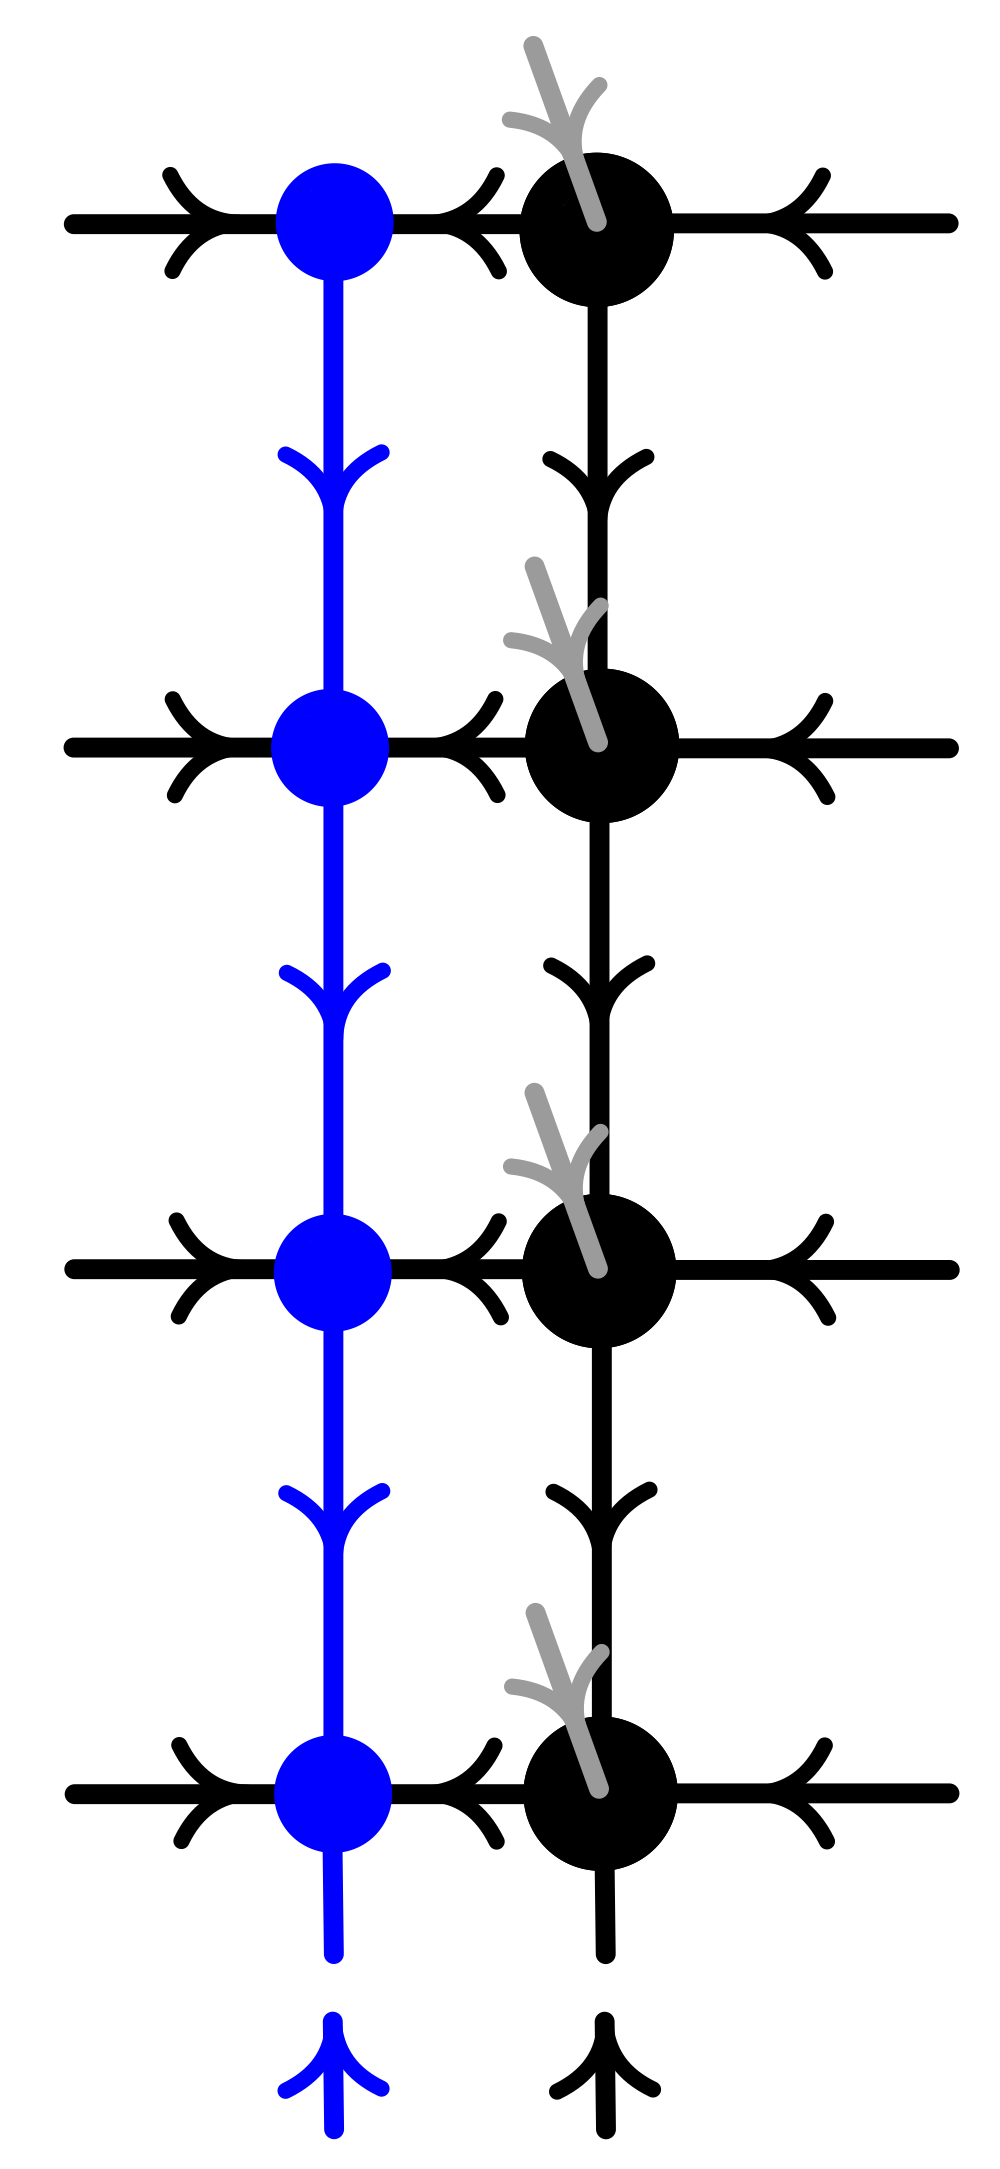
\includegraphics[height=3.5cm]{mm1.png}} 
	\:=\:
	\raisebox{-0.5\height}{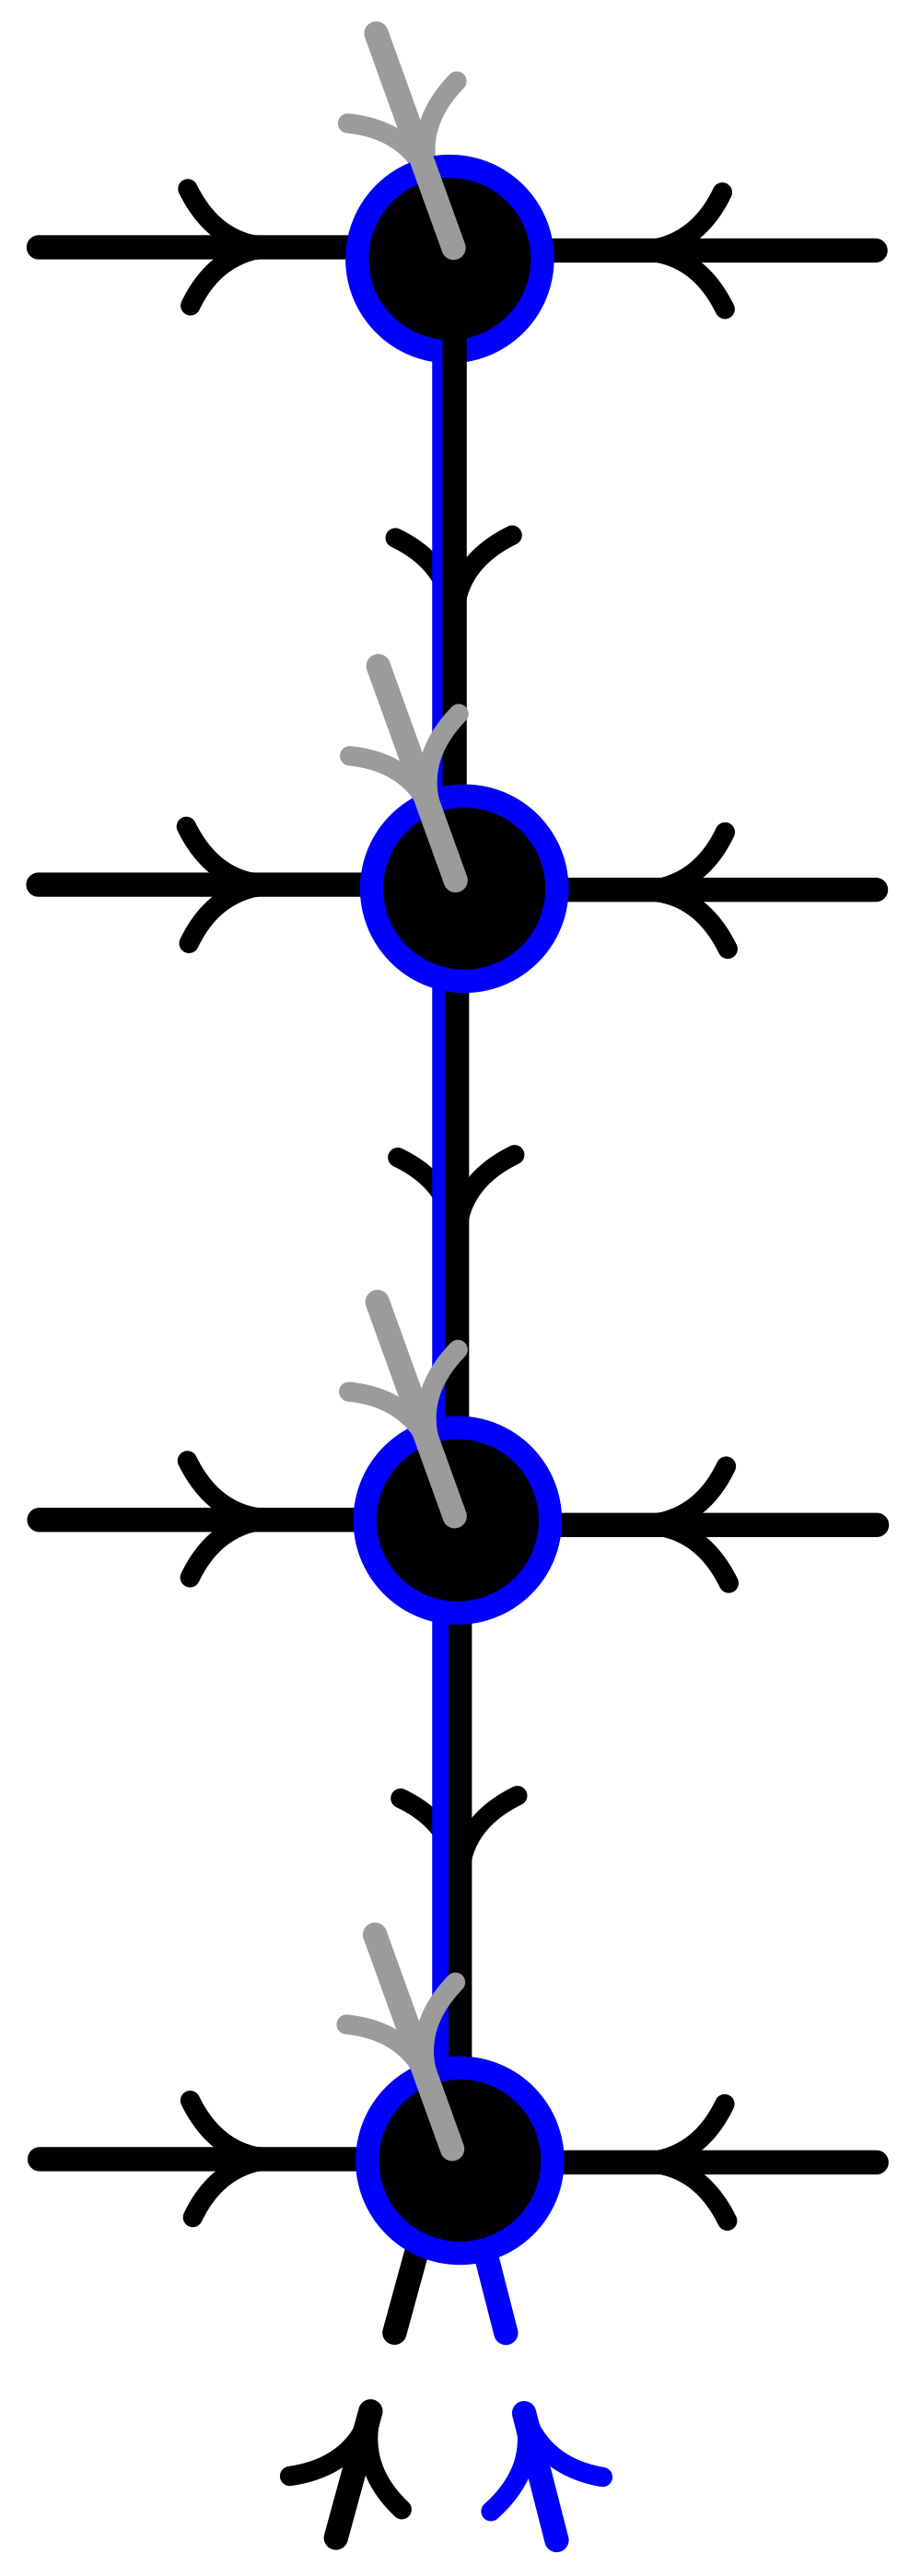
\includegraphics[height=3.5cm]{mm2.png}} 
	\: \approx \:
	\raisebox{-0.5\height}{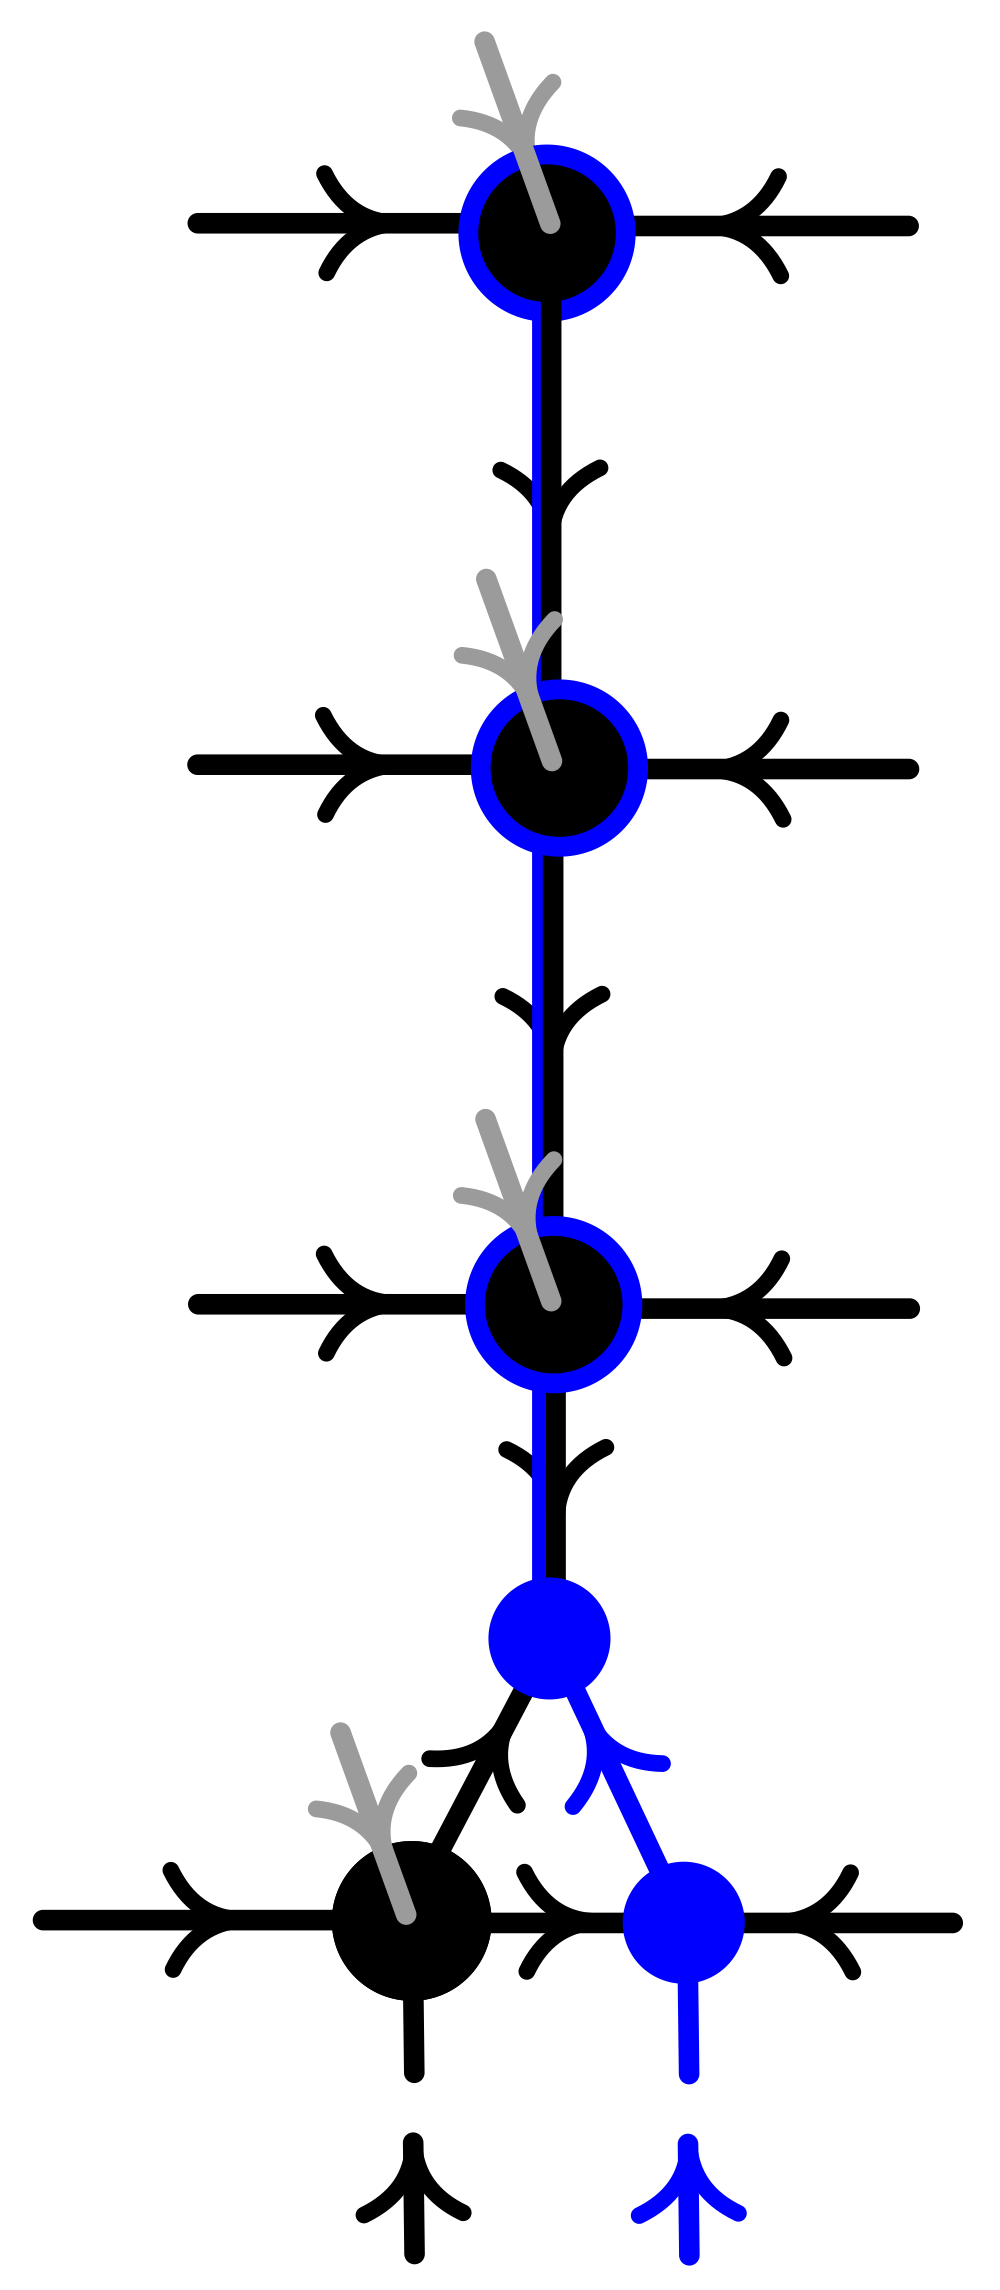
\includegraphics[height=3.5cm]{mm3.png}} 
	\:=\:
	\raisebox{-0.5\height}{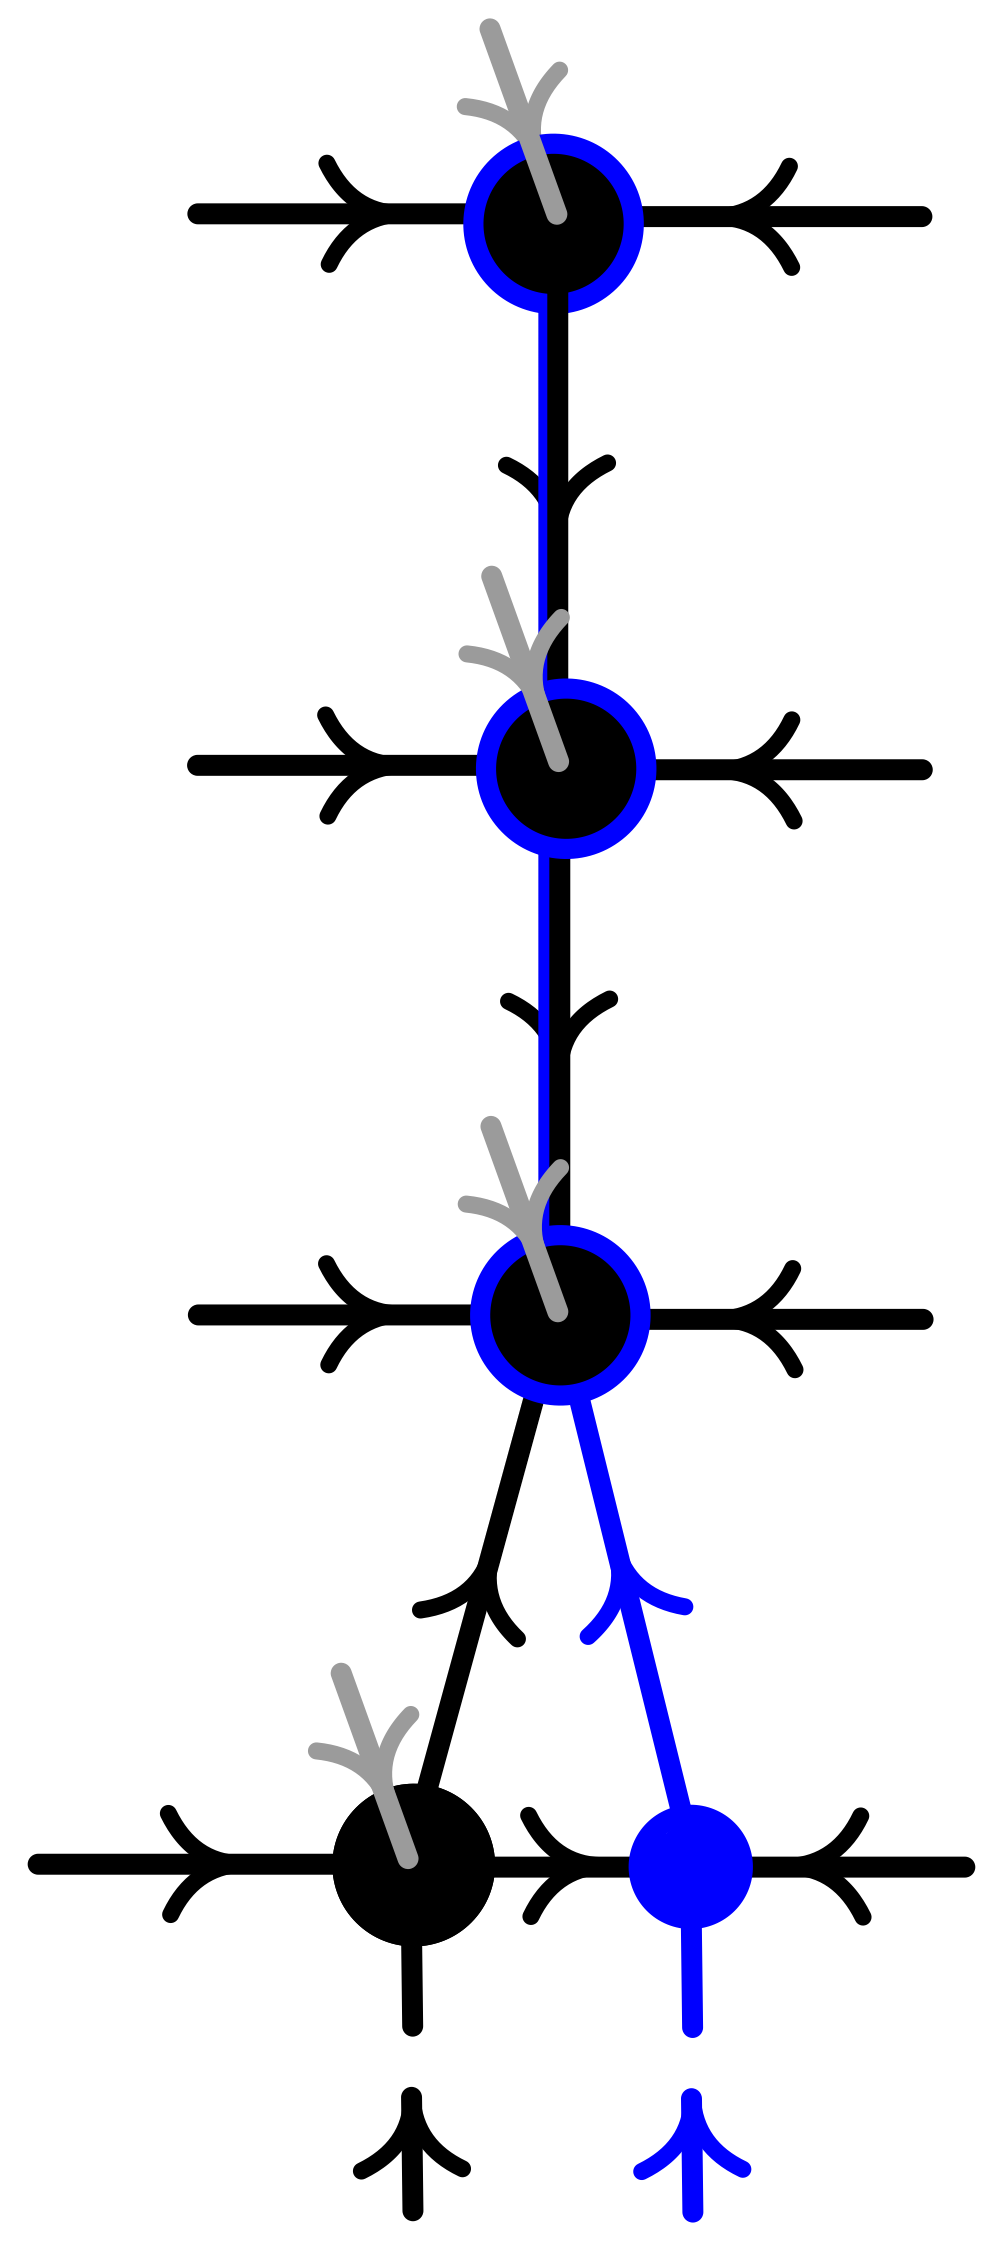
\includegraphics[height=3.5cm]{mm4.png}} 
	\: \approx \: \ldots \: \approx \:
	\raisebox{-0.5\height}{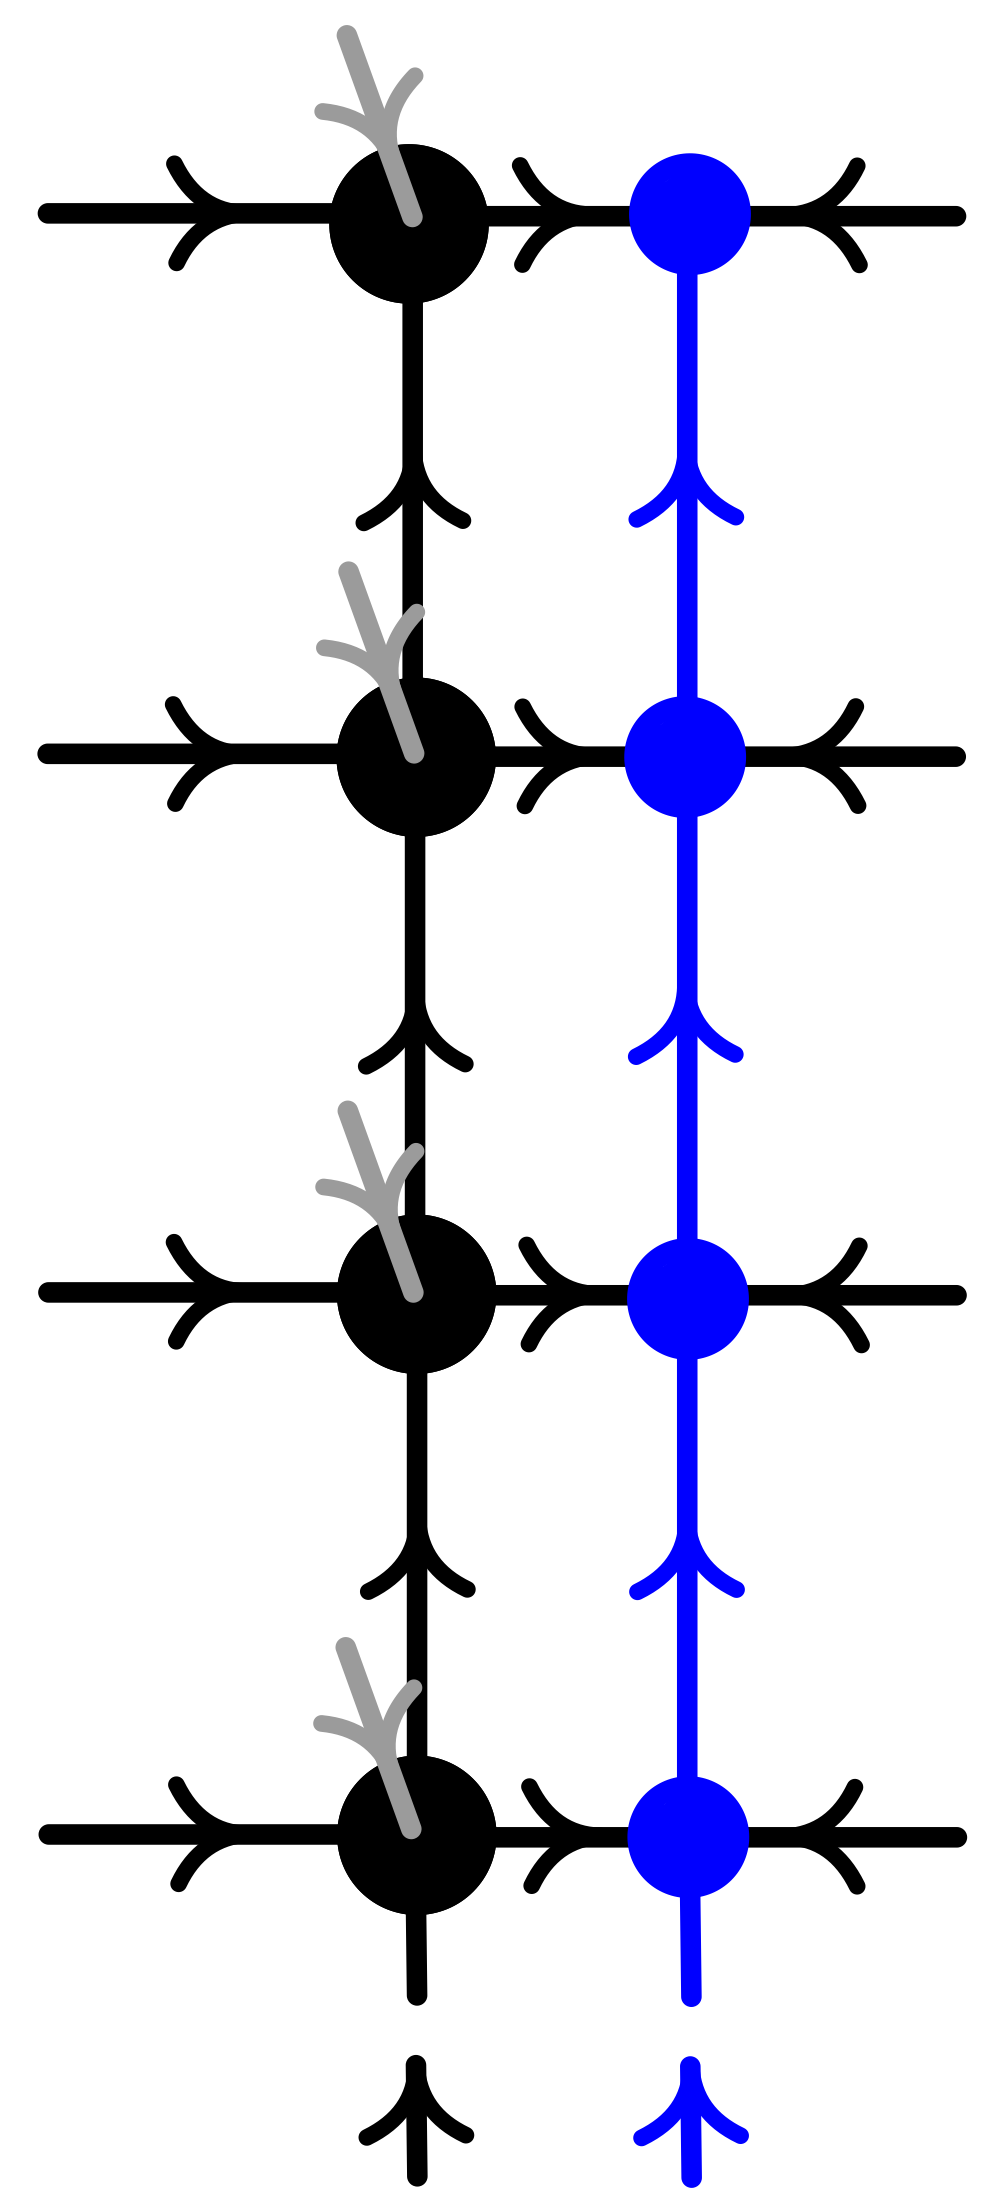
\includegraphics[height=3.5cm]{mm5.png}} \:.
\end{equation}
The crucial tripartite tensor decomposition works the same way as the one we described in \eqref{eq:YB} for the YB move. \\[0.5em]
\noindent It would be interesting to set up and test a quasiparticle excitation ansatz for these MM isoPEPS as well. Notably, our diagonal isoPEPS ansatz is not straightforwardly transferable. This is due to the fact that not all outgoing legs of the $A_L$-tensors are connected with the orthogonality column that is located right next to them. As a consequence, replacing one $A_L$ with $V_L X$---to fulfill the orthogonality conditions \eqref{eq:e_iso_peps_properties}---the perturbation $X$ cannot be absorbed into the orthogonality center. \\[0.5em]
\noindent Unlike the excitation ansatz, our newly proposed bulk-weighted boundary compression is directly applicable to MM isoPEPS. Regarding boundary compression in general and this new method in particular, it would be worthwhile to investigate potential performance differences between the two lattice choices. \\[1em]

\noindent \underline{Infinite version with definite momentum} \\[0.5em]
In order to put our quasiparticle excitations in a plane wave superposition with definite momentum, we need a uniform version of the isoPEPS. For the conventional MM isoPEPS, infinite columns were established in \cite{wu2023two}, but an infinite extension in both directions is still missing (for MM and diagonal isoPEPS). It requires finding a fixed-point solution of $A_L C = C A_R$, the column analog of the tensor equation that appeared for the canonical form of uMPS in section \ref{sec:canonical_form_area_law}. There, we could reach convergence with iterative positive QR decompositions \eqref{eq:iterative_qr}. There is no a priori reason to achieve the same with repeatedly applying the MM or YB move. \\[0.5em]

\noindent \underline{Application to more challenging models} \\[0.5em]
In this thesis, we benchmarked all algorithms on the TFI model. Naturally, having established that they work on this comparatively simple model, it is desirable to apply them to more challenging systems, such as quantum spin liquids (QSL) mentioned in the introduction. Of special interest are numerical predictions about quantities that are directly accessible in experiments on candidate materials. Inelastic neutron scattering, for instance, measures the dynamical structure factor. It results from a space-time Fourier transformation of the dynamical two-point correlation function $C(n, t)$ for a local operator $O$:
\begin{equation}
	S(p, \omega) = \frac{1}{2 \pi} \int_{-\infty}^{\infty} dt \sum_n e^{i(\omega t - p \cdot n)} C(n, t) 
	\:\: \text{ with } C(n, t) = \langle \psi_0 \vert e^{iHt} O^{[n]} e^{-iHt} O^{[0]} \vert \psi_0 \rangle.
\end{equation}
In the following, we sketch two possible routes for computing $S(p, \omega)$ with tensor network methods.
\begin{enumerate}
	\item[1)] Lowest-lying excitation branch from quasiparticle ansatz \\[0.5em]
	By projecting the time evolution onto all excited states of $H$, we can simplify the correlation function as
	\begin{equation}
		C(n, t) = \sum_X e^{-i(E_X - E_0)t} \langle \psi_0 \vert O^{[n]} \vert \psi_X \rangle \langle \psi_X \vert O^{[0]} \vert \psi_0 \rangle.
	\end{equation}
	We perform the Fourier transformation in time, denote with $\epsilon_X = E_X - E_0$ the energy above the ground state and end up with
	\begin{equation}
		S(p, \omega) = \sum_{X, n} e^{-ip \cdot n} \langle \psi_0 \vert O^{[n]} \vert \psi_X \rangle \langle \psi_X \vert O^{[0]} \vert \psi_0 \rangle \delta(\omega - \epsilon_X).
	\end{equation}
	With the tangent space ansatz \eqref{eq:e_iso_peps}, we can only capture the isolated branch of single quasiparticle excitations, corresponding to a subset of terms in the sum over $X$ in $S(p, \omega)$. For an overlap $\langle \psi_0 \vert O^{[n]} \vert \psi_X \rangle$---that contributes to the spectral weight at momentum $p$ after the Fourier sum---all states in the superposition $\vert \psi_X \rangle$, which have the excitation tensor left of the operator $O^{[n]}$, can be neglected due to the ground state orthogonality condition \eqref{eq:e_iso_peps_properties} 1). The nonzero terms, where the excitation tensors are right of the operator $O^{[n]}$, can be computed with the compressed bMPS \eqref{eq:RB}.
	\item[2)] Full excitation spectrum from time evolution \\[0.5em]
	Alternatively, we can compute the correlation function $C(n, t)$ explicitly by (i) finding a ground state approximation $\ket{\psi_0}$, (ii) applying the local operator $O^{[0]}$, (iii) time-evolving the perturbed state with $e^{-iHt}$ and (iv) computing the overlap with $O^{[n]}\ket{\psi_0}$:
	\begin{equation}
		C(n, t) = e^{iE_0t} \langle \psi_0 \vert O^{[n]} \underbrace{e^{-iHt} O^{[0]} \vert \psi_0 \rangle}_{= \ket{\psi(t)}} 
		= e^{iE_0t} \langle \psi_0 \vert O^{[n]} \vert \psi(t) \rangle.
	\end{equation}
	Then, we perform the Fourier transformation in space and time (where we multiply the time signal by a Gaussian window function to suppress artifacts arising from the finite time cutoff). In contrast to the quasiparticle ansatz, the time evolution accounts for the full excitation spectrum and can thus capture two particle scattering continua in $S(p, \omega)$. The downside is typically a higher computational cost.
\end{enumerate}
In \cite{drescher2023dynamical} these two approaches show excellent agreement for the dynamical spin structure factor of the highly frustrated, anti-ferromagnetic $J_1$-$J_2$ Heisenberg model on a triangular lattice. They were implemented for an MPS on a cylindrical geometry. It would be interesting to see whether the obtained results can be reproduced with isoPEPS methods. Since $\text{TEBD}^2$ (at least without the use of SWAP gates) cannot be applied to models with next-nearest-neighbor interactions (such as the $J_1$-$J_2$ model), a 2D version of TDVP is another further research direction. \\[1em]

\noindent \underline{Towards a tangent space projector and TDVP} \\[0.5em]
The time-dependent variational principle (TDVP) projects the right hand side of the Schrödinger equation onto the tangent space of the manifold at the current state:
\begin{equation}
	\frac{\mathrm{d}}{\mathrm{d}t} \ket{\psi(A)} = -i P_{\ket{\psi(A)}} H \ket{\psi(A)}.
\end{equation}
This ensures that the state never leaves the manifold and can be described in terms of time-evolving tensors $\ket{\psi(A_t)}$ \cite{haegeman2016unifying}. The following advantages over TEBD make TDVP particularly powerful for accurate long-time evolution \cite{haegeman2013post}:
\begin{itemize}
	\item In its one-site formulation, TDVP exactly conserves the energy (and other symmetries of the Hamiltonian).
	\item TDVP does not rely on splitting the Hamiltonian into local gates. Consequently, it avoids the Trotter error present in TEBD and can be applied to Hamiltonians with long-range interactions. 
\end{itemize}
To implement TDVP for isoPEPS, we need an expression for the projector $P_{\ket{\psi(A_L, C)}}$ onto the tangent space, which is spanned by the states $\ket{\psi(B, D; A_L, C)}$ \eqref{eq:iso_peps_tangent_vector}. Our parametrization $(B, D)(X)$ according to (\ref{eq:e_iso_peps_VL_plus}, \ref{eq:e_iso_peps_VD}) ensures an identity norm matrix \eqref{eq:e_iso_peps_properties} and allows us to solve the minimization problem $\argmin_X \Vert \psi(X; A_L, C) - \varphi \Vert^2$ for an arbitrary state $\varphi$ easily and express its projection onto the tangent space as
\begin{equation}
	P_{\ket{\psi(A_L, C)}} \ket{\varphi} = \ket{\psi(X_{\varphi}; A_L, C)}
	\text{ with } X_{\varphi} = \partial_{\overline{X}} \langle \psi(\overline{X}; \overline{A}_L, \overline{C}) \vert \varphi \rangle.
\end{equation}
To make a statement about the exactness of $P_{\ket{\psi(A_L, C)}}$, we have to ultimately find all gauge transformations (in addition to \eqref{eq:e_iso_peps_gauge}) that leave the tangent space vector $\ket{\psi(B, D; A_L, C)}$ invariant.